\begin{name}
	{\tenchude}
	{THPT Nguyễn Gia Thiều - Hà Nội}
	{LỚP TOÁN THẦY PHÁT}
	{Si tu n’aimes pas ce que tu récoltes. Alors change ce que tu sèmes.}
\end{name}

\TN
\setcounter{ex}{0}
\Opensolutionfile{ans}[ans/ans-2-TT3-SGDDT-HaNoi-2526]
%1
\begin{ex}%[0D3N1-6]
	Cho hàm số $f(x)$ xác định trên $\mathbb{R}$ thỏa mãn đồng thời hai điều kiện: $f(x)$ là hàm số lẻ và $f(x) = x^2$ với mọi $x \le 0$. Giá trị của $f(2)$ bằng
	\choice
	{\True $-4$}
	{$-2$}
	{$0$}
	{$4$}
	\loigiai{
		Vì $f(x)$ là hàm số lẻ nên $f(2) = -f(-2)$.\\
		Với $x = -2 \le 0$, ta có $f(-2) = (-2)^2 = 4$.\\
		Vậy $f(2) = -4$.
	}
\end{ex}
%2
\begin{ex}%[1D1N5-3]
	Tập nghiệm của phương trình $\cot x = -1$ là
	\choice
	{$S = \left\{ \dfrac{\pi}{4} + k2\pi \mid k \in \mathbb{Z} \right\}$}
	{$S = \left\{ \dfrac{\pi}{4} + k\pi \mid k \in \mathbb{Z} \right\}$}
	{$S = \left\{ \dfrac{3\pi}{4} + k2\pi \mid k \in \mathbb{Z} \right\}$}
	{\True $S = \left\{ \dfrac{3\pi}{4} + k\pi \mid k \in \mathbb{Z} \right\}$}
	\loigiai{
		Ta có $\cot x = -1\Leftrightarrow \cot x =\cot \left(\dfrac{3\pi}{4}\right)\Leftrightarrow x = \dfrac{3\pi}{4} + k\pi$, ($k \in \mathbb{Z}$).\\
		Vậy $S = \left\{ \dfrac{3\pi}{4} + k\pi \mid k \in \mathbb{Z} \right\}$.
	}
\end{ex}
%3
\begin{ex}%[2D1N2-1]
	Giá trị cực tiểu của hàm số $y = 4x^3 - 6x^2 + 11$ bằng
	\choice
	{$0$}
	{$1$}
	{\True $9$}
	{$11$}
	\loigiai{
		Ta có $y' = 12x^2 - 12x = 12x(x-1)$ và
		$y' = 0 \Leftrightarrow \hoac{&x=0\\&x=1.}$\\
		Bảng biến thiên
		\begin{center}
			
\begin{tikzpicture}
				\tkzTabInit[nocadre=false, lgt=1, espcl=2.5]
				{$x$/0.6, $y'$/0.6, $y$/2}
				{$-\infty$, $0$, $1$, $+\infty$}
				\tkzTabLine{, +, 0, -, 0, +, }
				\tkzTabVar{-/ $-\infty$, +/ $11$, -/ $9$, +/ $+\infty$}
				\path (0,0) node{\hypersetup{hidelinks}\href{tpSzVVc}{ }};
			\end{tikzpicture}
		\end{center}
		Giá trị cực tiểu của hàm số là $y(1) = 4\cdot 1^3 - 6\cdot 1^2 + 11 = 9$.
	}
\end{ex}
%4
\begin{ex}%[2D1N1-1]
	Hàm số $y = -2x^3 + 9x^2 + 24x - 114$ đồng biến trên khoảng nào dưới đây?
	\choice
	{\True $(-1; 4)$}
	{$(-4; -1)$}
	{$(-\infty; -1)$}
	{$(4; +\infty)$}
	\loigiai{
		Ta có $y' = -6x^2 + 18x + 24$ và
		$y'=0\Leftrightarrow\hoac{&x=-1\\&x=4.}$\\
		Bảng biến thiên
		\begin{center}
			
\begin{tikzpicture}
				\tkzTabInit[nocadre=false, lgt=1, espcl=2.5]
				{$x$/0.6, $y'$/0.6, $y$/2}
				{$-\infty$, $-1$, $4$, $+\infty$}
				\tkzTabLine{, -, 0, +, 0, -, }
				\tkzTabVar{+/ $+\infty$, -/ $-114$, +/ $-83$, -/ $-\infty$}
			\end{tikzpicture}
		\end{center}
		Vậy hàm số đồng biến trên khoảng $(-1; 4)$.
	}
\end{ex}
%5
\begin{ex}%[2D1N3-1]
	\immini[thm]{
	Cho hàm số $f(x)$ liên tục trên $[-1; 5]$ và có đồ thị như hình vẽ bên (các điểm cực trị của đồ thị thể hiện rõ trên hình). Gọi $M$ và $m$ lần lượt là giá trị lớn nhất và nhỏ nhất của hàm số đã cho trên $[-1; 5]$. Giá trị của $M - m$ bằng
	\choice
	{$1$}
	{$4$}
	{\True $5$}
	{$6$}
	}
	{
	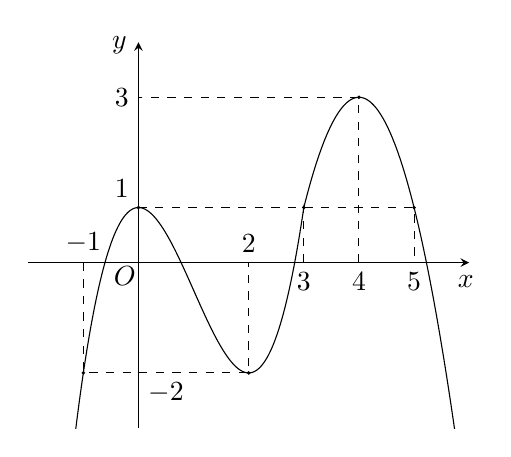
\begin{tikzpicture}[line cap=butt,line join=miter,>=stealth,scale=0.7]
		\tikzset{declare function={xmin=-2;xmax=6;ymin=-3;ymax=4;
				f(\x)=0.75*(\x)^3-2.25*(\x)^2+1;
				g(\x)=-2*(\x)^2+16*(\x)-29;
			},
			smooth,samples=450
		}
		\draw[->] (xmin,0)--(xmax,0) node[shift={(-100:7pt)},font=\normalsize]{$ x $};
		\draw[->] (0,ymin)--(0,ymax) node[shift={(190:7pt)},font=\normalsize]{$ y $};
		\fill (0,0) node[shift={(225:7pt)},font=\normalsize]{$ O $};
		\fill (-1,-2) circle(1pt); \fill (0,1) circle(1pt); \fill (2,-2) circle(1pt);
		\fill (3,1) circle(1pt); \fill (4,3) circle(1pt); \fill (5,1) circle(1pt);
		\draw[dashed] (-1,0)node[above]{$-1$}--(-1,-2)--(0,-2)node[below right]{$-2$}--(2,-2)--(2,0)node[above]{$2$} 
		(0,1)node[above left]{$1$}--(5,1)--(5,0)node[below]{$5$}
		(3,0)node[below]{$3$}--(3,1)
		(4,0)node[below]{$4$}--(4,3)--(0,3)node[left]{$3$}
		;
		\clip (xmin,ymin) rectangle (xmax,ymax);
		\draw  plot[domain=xmin:3.01] (\x, {f(\x)});
		\draw  plot[domain=3:xmax] (\x, {g(\x)});
	\end{tikzpicture}	
	}
	\loigiai{
		Dựa vào đồ thị hàm số trên đoạn $[-1; 5]$, ta thấy\\
		Giá trị lớn nhất $M = 3$ tại $x = 4$.\\
		Giá trị nhỏ nhất $m = -2$ tại $x = 2$.\\
		Vậy $M - m = 3 - (-2) = 5$.
	}
\end{ex}
%6
\begin{ex}%[2D1N4-1]
	Tiệm cận ngang của đồ thị hàm số $y = \dfrac{2x-4}{x+2}$ là đường thẳng có phương trình
	\choice
	{\True $y = 2$}
	{$y = -2$}
	{$x = 2$}
	{$x = -2$}
	\loigiai{
		Tập xác định $\mathscr{D}=\mathbb{R}\setminus\{-2\}$.\\
		Ta có $\lim\limits_{x \to +\infty} \dfrac{2x-4}{x+2} = 2$ và $\lim\limits_{x \to -\infty} \dfrac{2x-4}{x+2} = 2$.\\
		Vậy tiệm cận ngang của đồ thị hàm số là đường thẳng $y = 2$.
	}
\end{ex}
%7
\begin{ex}%[2D3H2-3]
	Hướng tới kỳ thi tốt nghiệp THPT, học sinh hai lớp chất lượng cao 12A và 12B của trường NQH tham gia một kỳ thi thử môn Toán. Kết quả (số học sinh) theo các khoảng điểm như sau
	\begin{center}
		\begin{tabular}{|l|c|c|c|c|c|}
			\hline
			Điểm & $[5; 6)$ & $[6; 7)$ & $[7; 8)$ & $[8; 9)$ & $[9; 10]$ \\ \hline
			Lớp $12$A& $5$ & $11$ & $13$ & $8$ & $3$ \\ \hline
			Lớp $12$B & $3$ & $5$ & $22$ & $2$ & $8$ \\ \hline
		\end{tabular}
	\end{center}
	Khi so sánh, các giá trị điểm trung bình và độ phân tán điểm đo bằng độ lệch chuẩn của hai lớp. Nhận định nào sau đây đúng?
	\choice
	{Lớp 12B có điểm trung bình cao hơn và độ phân tán điểm cao hơn lớp 12A}
	{Lớp 12B có điểm trung bình cao hơn và độ phân tán điểm thấp hơn lớp 12A}
	{\True Lớp 12B có điểm trung bình cao hơn lớp 12A, và độ phân tán điểm của hai lớp bằng nhau}
	{Lớp 12A có điểm trung bình cao hơn lớp 12B, và độ phân tán điểm của hai lớp bằng nhau}
	\loigiai{
		\begin{center}
			\begin{tabular}{|l|c|c|c|c|c|}
				\hline
				Điểm & $[5; 6)$ & $[6; 7)$ & $[7; 8)$ & $[8; 9)$ & $[9; 10]$ \\
				\hline
				Giá trị đại diện&$5{,}5$ & $6{,}5$ & $7{,}5$ & $8{,}5$ & $9{,}5$ \\ \hline
				Lớp $12$A& $5$ & $11$ & $13$ & $8$ & $3$ \\ \hline
				Lớp $12$B & $3$ & $5$ & $22$ & $2$ & $8$ \\ \hline
			\end{tabular}
		\end{center}
		\begin{itemize}
			\item Lớp 12A
			\begin{itemize}
				\item Số học sinh lớp 12A: $n_A = 40$.
				\item Điểm trung bình lớp 12A: $\overline{x}_A = \dfrac{5 \cdot 5{,}5 + 11 \cdot 6{,}5 + 13 \cdot 7{,}5 + 8 \cdot 8{,}5 + 3 \cdot 9{,}5}{40} = 7{,}325$.
				\item Phương sai $s_A^2 =\dfrac{5 \cdot 5{,}5^2 + 11 \cdot 6{,}5^2 + 13 \cdot 7{,}5^2 + 8 \cdot 8{,}5^2 + 3 \cdot 9{,}5^2}{40}-  \overline{x}_A^2 = 54{,}9 - 7{,}325^2 = 1{,}244375$.
			\end{itemize}
			\item Lớp 12B
			\begin{itemize}
				\item Số học sinh lớp 12B: $n_B = 40$.
				\item Điểm trung bình lớp 12B: $\overline{x}_B = \dfrac{3 \cdot 5{,}5 + 5 \cdot 6{,}5 + 22 \cdot 7{,}5 + 2 \cdot 8{,}5 + 8 \cdot 9{,}5}{40} = 7,675$.
				\item phương sai $s_B^2 = \dfrac{3 \cdot 5{,}5^2 + 5 \cdot 6{,}5^2 + 22 \cdot 7{,}5^2 + 2 \cdot 8{,}5^2 + 8 \cdot 9{,}5^2}{40}-\overline{x}_B^2 = 60{,}15 - 7{,}675^2 = 1{,}244375$.
			\end{itemize}
		\end{itemize}
		Vậy $\overline{x}_B > \overline{x}_A$ và độ lệch chuẩn hai lớp bằng nhau $s_A = s_B = \sqrt{1,244375}$.
	}
\end{ex}
%8
\begin{ex}%[2H2N1-2]
	% \immini[thm]{
	Cho hình hộp $ABCD.A'B'C'D'$. Khẳng định nào trong các khẳng định sau đây là đúng?
	\choice
	{$\overrightarrow{BC} + \overrightarrow{BA} + \overrightarrow{BD'} = \overrightarrow{BB'}$}
	{\True $\overrightarrow{AD} + \overrightarrow{D'C'} + \overrightarrow{CC'} = \overrightarrow{AC'}$}
	{$\overrightarrow{BC} + \overrightarrow{BA} = \overrightarrow{D'A'} + \overrightarrow{D'C'}$}
	{$\overrightarrow{BA} + \overrightarrow{DD'} + \overrightarrow{BD'} = \overrightarrow{BC}$}
	% }
	% {
	% \begin{tikzpicture}[declare function={a=5;b=3;h=4;},scale=0.7]
	% 	\path(0,0) coordinate(A)
	% 	(a,0) coordinate(B)
	% 	(45:b) coordinate(D)
	% 	($(D)+(100:h)$) coordinate(D');
	% 	\path($(B)-(A)+(D)$) coordinate(C);
	% 	\path($(D')-(D)+(A)$) coordinate(A')
	% 	($(D')-(D)+(B)$) coordinate(B')
	% 	($(D')-(D)+(C)$) coordinate(C');
	% 	\draw[dash pattern=on 2pt off 1.5pt](A)--(D)--(D') (D)--(C);
	% 	\draw (B)--(C)--(C') (A)--(B)--(B')--(A')--cycle (D')--(A')--(B')--(C')--cycle;
	% 	\foreach\t/\g in{A/-90,B/-90,C/0,D/180,A'/90,B'/90,C'/90,D'/90}{
	% 		\draw[fill=black](\t)circle(1pt)node[shift={(\g:7pt)},font=\scriptsize]{$\t$};
	% 	}
	% \end{tikzpicture}
	% }
	\loigiai{
		Ta có $\overrightarrow{AD} + \overrightarrow{D'C'} + \overrightarrow{CC'} = \overrightarrow{AD} + \overrightarrow{DC} + \overrightarrow{CC'} = \overrightarrow{AC} + \overrightarrow{CC'} = \overrightarrow{AC'}$.
	}
\end{ex}
%9
\begin{ex}%[2H2H2-4]
	Trong không gian $Oxyz$; cho hai véc-tơ $\overrightarrow{m} = (1; 1; 4)$, $\overrightarrow{n} = (4; 1; 1)$. Véc-tơ nào dưới đây vuông góc với cả hai véc-tơ $\overrightarrow{m}$ và $\overrightarrow{n}$?
	\choice
	{$\overrightarrow{a} = (1; 5; 1)$}
	{\True $\overrightarrow{b} = (1; -5; 1)$}
	{$\overrightarrow{c} = (1; 5; -1)$}
	{$\overrightarrow{d} = (-1; 5; 1)$}
	\loigiai{
		Véc-tơ vuông góc với cả $\overrightarrow{m}$ và $\overrightarrow{n}$ có phương cùng phương với tích có hướng $\left[\overrightarrow{m}, \overrightarrow{n}\right]$.\\
		Ta có $\left[\overrightarrow{m}, \overrightarrow{n}\right] = (1\cdot 1 - 4\cdot 1; 4\cdot 4 - 1\cdot 1; 1\cdot 1 - 1\cdot 4) = (-3; 15; -3)$.\\
		Véc-tơ này cùng phương với $\overrightarrow{b} = (1;- 5;1)$.
	}
\end{ex}
%10
\begin{ex}%[1H4H1-3]
	Cho hình chóp $S.ABCD$ có đáy là hình thang ($AD \parallel BC$, $AD > BC$). Gọi $I$ là giao điểm của $AB$ và $CD$, $O$ là giao điểm $AC$ và $BD$. Giao tuyến của hai mặt phẳng $(SAD)$ và $(SBC)$ là đường thẳng
	\choice
	{$SI$}
	{$SO$}
	{$IO$}
	{\True đi qua $S$ và song song với $AD$}
	\loigiai{
		\immini[thm]{
		Ta có $\heva{&S\in (SAD)\cap (SBC)\\&AD \subset (SAD)\\&BC \subset (SBC)\\&AD \parallel BC}
		\Rightarrow (SAD)\cap (SBC)=d$ \\với $d$ là đường thẳng đi qua $S$ và song song với $AD$ (và $BC$).}
		{	
		\begin{tikzpicture}[declare function={gocx=80; goc=-150; a=5; b=a/2; h=4;},scale=0.7]
			\path (0,0) coordinate (A)--+(gocx:h) coordinate (S)
			(a,0) coordinate (D)
			(goc:b) coordinate (B')
			+(a,0) coordinate (C)
			($(B')!.6!(C) $) coordinate (B)
			($(S)+(D)-(A)$) coordinate (x)
			;
			\draw[dashed] (A)--(D);
			\draw (S)--(A)--(B)--(C)--(D)--(S)--(C) (S)--(B)
			($(S)!-0.2!(x)$)--($(x)!-0.2!(S)$)node[right]{$d$}
			;
			\foreach \x/\goc in {S/90,A/150,B/180,C/-60,D/0}
			\draw[fill=black] (\x) node[shift={(\goc:7pt)},font=\scriptsize]{$\x$} circle (1pt);
			\path (0,0) node{\hypersetup{hidelinks}\href{tpSzVVc}{ }};
		\end{tikzpicture}
	}
	}
\end{ex}
%11
\begin{ex}%[1H8H4-2]
	Cho hình chóp $S.ABCD$ có đáy $ABCD$ là hình chữ nhật và $SA \perp AD$. Khi đó ta có
	\choice
	{$(SAC) \perp (SAB)$}
	{$(SCD) \perp (SAB)$}
	{$(SBD) \perp (SAB)$}
	{\True $(SBC) \perp (SAB)$}
	\loigiai{
		\immini[thm]{
		Ta có $\heva{&BC\parallel AD\\&AD\perp SA}\Rightarrow BC\perp SA$.\\
		 Khi đó  $\heva{&BC \perp AB\, (\text{do}\, ABCD\, \text{là hình chữ nhật})\\&BC\perp SA}
		 \Rightarrow BC\perp (SAB)$.\\ 
		 Mà $BC \subset (SBC)$ nên $(SBC) \perp (SAB)$.}
		{
		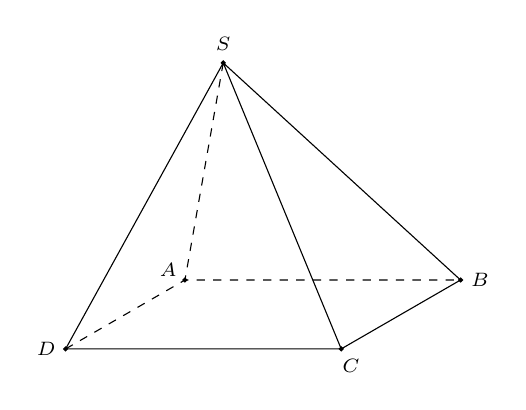
\begin{tikzpicture}[declare function={gocx=80; goc=-150; a=5; b=a/2; h=4;},scale=0.7]
			\path (0,0) coordinate (A)--+(gocx:h) coordinate (S)
			(a,0) coordinate (B)
			(goc:b) coordinate (D)
			+(a,0) coordinate (C);
			\draw[dashed] (S)--(A) (D)--(A)--(B);
			\draw (S)--(D)--(C)--(S)--(B)--(C)--cycle;
			\foreach \x/\goc in {S/90,A/150,B/0,C/-60,D/-180}
			\draw[fill=black] (\x) node[shift={(\goc:7pt)},font=\scriptsize]{$\x$} circle (1pt);
		\end{tikzpicture}
	}		
	}
\end{ex}

\begin{ex}%[2D3H1-3]
	Hướng tới kỳ thi tốt nghiệp THPT, học sinh hai lớp 12C và 12D tham gia thi thử. Kết quả như sau:
	\begin{center}
		\begin{tabular}{|l|c|c|c|c|c|}
			\hline
			Điểm & $[5; 6)$ & $[6; 7)$ & $[7; 8)$ & $[8; 9)$ & $[9; 10]$ \\ \hline
			Lớp 12C & 7 & 9 & 10 & 5 & 9 \\ \hline
			Lớp 12D & 4 & 6 & 23 & 10 & 2 \\ \hline
		\end{tabular}
	\end{center}
	So sánh giá trị điểm trung bình và độ rộng khoảng tứ phân vị. Nhận định nào đúng?
	\choice
	{Điểm trung bình hai lớp bằng nhau và độ phân tán điểm của hai lớp bằng nhau}
	{\True Điểm trung bình hai lớp bằng nhau và độ phân tán điểm lớp 12C lớn hơn lớp 12D}
	{Điểm trung bình hai lớp bằng nhau và độ phân tán điểm lớp 12D lớn hơn lớp 12C}
	{Điểm trung bình lớp 12C cao hơn lớp 12D và độ phân tán điểm lớp 12C lớn hơn lớp 12D}
	\loigiai{
		Lớp $12$C
		\begin{itemize}
			\item Số học sinh là $40$.
			\item Số điểm trung bình $\overline{x}_C = \dfrac{7 \cdot 5{,}5 + 9 \cdot 6{,}5 + 10 \cdot 7{,}5 + 5 \cdot 8{,}5 + 9 \cdot 9{,}5}{40} = 7{,}5$.
			\item Tứ phân vị thứ nhất $Q_1$ là giá trị đứng ở vị trí thứ $10$.  \\
				Giá trị này thuộc lớp $[6;7)$ nên $Q_1=6+\dfrac{10-7}{9}\cdot (7-1)=\dfrac{19}{3}$.
			\item Tứ phân vị thứ ba $Q_3$ là giá trị đứng ở vị trí thứ $30$.  \\
			Giá trị này thuộc lớp $[8;9)$ nên $Q_3=8+\dfrac{30-(7+9+10)}{5}\cdot (9-8)=\dfrac{44}{5}$.\\
			Do đó $\Delta Q_C=Q_3-Q_1=\dfrac{44}{5}-\dfrac{19}{3}=\dfrac{37}{15}\approx2{,}47$.
		\end{itemize}
		Lớp $12$D
		\begin{itemize}
			\item Số học sinh là $n=45$.
			\item Số điểm trung bình $\overline{x}_D = \dfrac{4 \cdot 5{,}5 + 6 \cdot 6{,}5 + 23 \cdot 7{,}5 + 10 \cdot 8{,}5 + 2 \cdot 9{,}5}{45} = 7{,}5$.
			\item Ta có $\dfrac{n}{4}=\dfrac{45}{4}=11{,}25$. Vì $4+6<\dfrac{n}{4}<4+6+23$ nên
			$Q_1$  thuộc lớp $[7;8)$. \\
			Ta có $Q_1=7+\dfrac{11{,}25-10}{23}\cdot 1=\dfrac{649}{92}$.
			\item Ta có $\dfrac{3n}{4}=\dfrac{3\cdot 45}{4}=33{,}75$. Vì $4+6+23<\dfrac{3n}{4}<4+6+23+10$ nên
			$Q_3$ thuộc lớp $[8;9)$. \\
			Ta có $Q_3=8+\dfrac{33{,}75-33}{10}\cdot 1=\dfrac{323}{40}$.
			\item $\Delta Q_D=Q_3-Q_1=\dfrac{323}{40}-\dfrac{649}{92}=\dfrac{371}{920}\approx 0{,}40$.
		\end{itemize}
		Vậy điểm trung bình hai lớp bằng nhau và độ phân tán điểm của lớp $12$C lớn hơn lớp $12$D.
	}
\end{ex}

\cauds
\begin{ex}%[12-EX-de-So-2026, Lê Hồng Phi]%[2D3H1-4]
	Một công ty giao hàng nhanh trong thành phố đã xây dựng một thuật toán giao hàng tối ưu. Để kiểm chứng, giám đốc yêu cầu ghi nhận thời gian giao của từng đơn hàng trong mẫu $100$ đơn chạy thử. Số liệu được thống kê trong bảng sau:
	\begin{center}
		\begin{tabular}{|l|c|c|c|c|c|}
			\hline
			Thời gian (phút) & $[10; 20)$ & $[20; 30)$ & $[30; 40)$ & $[40; 50)$ & $[50; 60]$ \\
			\hline
			Số đơn & $15$ & $40$ & $25$ & $12$ & $8$ \\
			\hline
		\end{tabular}
	\end{center}
	\choiceTF
	{\True Độ phân tán của thời gian giao hàng, ước lượng bằng khoảng biến thiên mẫu số liệu, là $50$ phút}
	{\True Một nửa số đơn hàng (trung vị ước lượng của mẫu số liệu) được giao xong không quá $28$ phút $45$ giây}
	{Thời gian giao hàng phổ biến nhất (giá trị mốt của mẫu số liệu tính theo công thức) bằng $25$ phút}
	{\True Công ty có chính sách niêm yết phí ship $20\,000$ đồng cho mỗi đơn. Cam kết nếu giao từ 40 phút trở lên, khách hàng không phải trả phí ship và nhận thêm $60\,000$ đồng tiền bồi thường từ công ty. Sau đợt chạy thử $100$ đơn này, tổng tiền phí ship thu được vẫn lớn hơn tổng số tiền bồi thường công ty phải chi trả}
	\loigiai{
		Ta có bảng tần số ghép nhóm như sau
		\begin{center}
			\begin{tabular}{|l|c|c|c|c|c|}
				\hline
				Thời gian (phút) & $[10; 20)$ & $[20; 30)$ & $[30; 40)$ & $[40; 50)$ & $[50; 60]$ \\
				\hline
				Số đơn & $15$ & $40$ & $25$ & $12$ & $8$ \\
				\hline
				Tần số tích lũy & $15$ & $55$ & $80$ & $92$ & $100$\\
				\hline
			\end{tabular}
		\end{center}
		Tổng số đơn hàng $n=100$.
		\begin{itemchoice}
			\itemch Khoảng biến thiên của mẫu số liệu ghép nhóm là $R=60-10=50$ (phút).
			\itemch
			Ta có $\dfrac{n}{2}=\dfrac{100}{2}=50$. \\
			Nhóm $[20;30)$ là nhóm đầu tiên có tần số tích lũy lớn hơn hoặc bằng $50$ nên nên trung vị thuộc nhóm $[20; 30)$. \\
			Ta có
			$M_e=20+\dfrac{50-15}{40}\cdot (30-20)=28{,}75$ (phút) $=28$ phút $45$ giây. \\
			Vậy một nửa số đơn hàng có thời gian giao không quá 28 phút 45 giây.
			\itemch Nhóm $[20;30)$ có tần số lớn nhất là $40$. \\
			Vậy $M_o=20+\dfrac{40-15}{2\cdot 40-15-25}\cdot (30-20)=26{,}25$ (phút).
			
			\itemch Đơn hàng giao từ $40$ phút trở lên thuộc hai nhóm $[40; 50)$ và $[50; 60]$. \\
			Số đơn hàng bị trễ là $12 + 8 = 20$ (đơn). \\
			Số đơn hàng giao đúng hạn (thu được phí ship) là $100-20=80$ (đơn).
			\begin{itemize}
				\item Tổng tiền phí ship thu được: $80 \times 20\,000 = 1\,600\,000$ (đồng).
				\item Tổng tiền bồi thường phải trả: $20 \times 60\,000 = 1\,200\,000$ (đồng).
			\end{itemize}
			Ta thấy $1\,600\,000 > 1\,200\,000$. Vậy tổng phí ship thu được lớn hơn tổng tiền bồi thường.
		\end{itemchoice}
	}
\end{ex}

\begin{ex}%[12-EX-de-So-2026, Lê Hồng Phi]%[2D4V2-6]
	\immini[thm]{Trong một thử nghiệm ô tô xuất phát từ trạng thái nghỉ. Người lái điều khiển xe đạt vận tốc cực đại tại $t=18$ giây, rồi giảm tốc và dừng hẳn. Toàn bộ quá trình kéo dài $50$ giây. Đồ thị vận tốc $v(t)$ (m/s) theo thời gian $t$ (s) như hình vẽ. Trong đó, đoạn $[0;24]$ đồ thị là một phần của parabol có đỉnh $I(18;27)$ và đi qua điểm $O$; trên đoạn $[24;50]$ đồ thị là đoạn thẳng $AB$, với $A(24;24)$ và $B(50;0)$.}{\begin{tikzpicture}[scale=0.1, >=stealth]
			\draw[->] (-5,0) -- (60,0) node[below] {$t(s)$};
			\draw[->] (0,-5) -- (0,35) node[left] {$v(t)$};
			\draw plot[domain=0:24] (\x, {-1/12*(\x-18)^2 + 27});
			\draw (24,24) -- (50,0);
			\draw[dashed] (18,0) node[below] {$18$} -- (18,27) -- (0,27) node[left] {$27$};
			\draw[dashed] (24,0) node[below] {$24$} -- (24,24) -- (0,24) node[left] {$24$};
			\node at (18,27) [above] {$I$}; \node at (24,24) [above right] {$A$}; \node at (50,0) [below] {$50$}; \node at (50,0) [above right] {$B$};
			\node at (0,0) [below left] {$O$};
	\end{tikzpicture}}
	\choiceTF
	{Trong $24$ giây đầu tiên, vận tốc của ô tô luôn tăng}
	{\True Trong $24$ giây đầu tiên, có một thời điểm mà gia tốc của ô tô bằng $2$ m/s$^2$}
	{\True Gọi giai đoạn $1$ là $[0;24]$, giai đoạn $2$ là $(24;50]$. Độ lớn gia tốc của ô tô ngay trước thời điểm kết thúc giai đoạn $1$ ($t=24$ giây) lớn hơn độ lớn gia tốc của ô tô trong suốt giai đoạn $2$ (từ $24$ giây đến $50$ giây)}
	{Quãng đường xe đi được trong $26$ giây cuối lớn hơn $70\%$ quãng đường xe chạy trong $24$ giây đầu tiên}
	\loigiai{
		Xác định hàm vận tốc.
		\begin{itemize}
			\item Giai đoạn $1$ ($0 \le t \le 24$): Đồ thị là parabol đỉnh $I(18; 27)$, đi qua $O(0;0)$. \\
			Phương trình có dạng $v_1(t)=a(t-18)^2+27$. \\
			Đồ thị đi qua gốc tọa độ $O(0;0)$ nên $0=a(0-18)^2+27 \Leftrightarrow a=-\dfrac{1}{12}$. \\
			Vậy $v_1(t)=-\dfrac{1}{12}(t-18)^2+27$.
			\item Giai đoạn $2$ ($24 \le t \le 50$): Đồ thị là đoạn thẳng đi qua $A(24; 24)$ và $B(50; 0)$.
			Phương trình đường thẳng có dạng $v_2(t)=mt+n$. \\
			Đồ thị đi qua $A$ và $B$ nên ta có hệ $$\heva{& 24m+n=24 \\ & 50m+n=0}\Leftrightarrow\heva{& m=-\dfrac{12}{13} \\ & n=\dfrac{600}{13}.}$$ Do đó $v_2(t)=-\dfrac{12}{13}t+\dfrac{600}{13}$.
		\end{itemize}
		\begin{itemchoice}
			\itemch Dựa vào đồ thị, ta thấy vận tốc tăng trên khoảng $(0; 18)$ và giảm trên khoảng $(18; 24)$.
			\itemch Trong $24$ giây đầu, gia tốc là $a_1(t)=v_1'(t)=-\dfrac{1}{6}(t-18)=3-\dfrac{t}{6}$. \\
			Xét phương trình $a_1(t)=2 \Leftrightarrow 3-\dfrac{t}{6}=2 \Leftrightarrow \dfrac{t}{6}=1 \Leftrightarrow t=6$. \\
			Vì $t=6 \in [0; 24]$ nên có thời điểm gia tốc bằng $2$ m/s$^2$.
			\itemch
			\begin{itemize}
				\item Ngay trước khi kết thúc giai đoạn $1$ thì
				$a_1(24)=3-\dfrac{24}{6}=-1$ m/s$^2$. Do đó, độ lớn $\left|a_1(24)\right|=1$ m/s$^2$.
				\item Trong giai đoạn $2$: Gia tốc là
				$a_2=-\dfrac{12}{13}$ m/s$^2$.
				Độ lớn $\left|a_2\right|=\dfrac{12}{13}$ m/s$^2$.
			\end{itemize}
			Vậy $\left|a_1(24)\right|=1 > \dfrac{12}{13}=\left|a_2\right|$.
			\itemch
			Quãng đường trong $24$ giây đầu là
			$S_1=\displaystyle\int\limits_0^{24}\left[-\dfrac{1}{12}(t-18)^2+27\right]\mathrm{d}t=480$ m. \\
			Quãng đường trong $26$ giây cuối (từ $t=24$ đến $t=50$) là
			$S_2=\displaystyle\int\limits_{24}^{50}\left(-\dfrac{12}{13}t+\dfrac{600}{13}\right)\mathrm{d}t=312$ m. \\
			Ta có $70\%$ của $S_1$ là $\dfrac{70}{100}\cdot 480 = 336$ (m). \\
			Vì $312 < 336$ nên quãng đường đi được trong $26$ giây cuối nhỏ hơn $70\%$ quãng đường đầu.
		\end{itemchoice}
	}
\end{ex}

\begin{ex}%[12-EX-de-So-2026, Lê Hồng Phi]%[2H5H2-8]
	Một phòng trưng bày nghệ thuật dạng hình hộp chữ nhật $ABCD. A'B'C'D'$ với kích thước: dài $AD=8$ mét, rộng $AB=6$ mét, cao $AA'=4$ mét. Kỹ sư thiết lập hệ trục tọa độ $Oxyz$ để số hóa căn phòng như sau: Gốc tọa độ $O(0;0;0)$ đặt tại $A$; các trục $Ox, Oy, Oz$ lần lượt trùng với các cạnh $AD, AB, AA'$ (chiều dương lần lượt từ $A$ đến $D$, từ $A$ đến $B$, từ $A$ đến $A'$). Hệ thống giám sát gồm một camera gắn tại tâm $S$ của mặt trần $A'B'C'D'$ và một cảm biến hồng ngoại gắn tại đỉnh $C$ (đỉnh đối diện với $A$ trên mặt sàn $ABCD$). Camera đang giám sát một bức tranh được treo chính giữa bức tường $CDD'C'$, gọi $P$ là tâm của bức tranh (cũng là tâm của hình chữ nhật $CDD'C'$).
	\choiceTF
	{\True Tọa độ vị trí lắp đặt camera là $S(4;3;4)$}
	{Khoảng cách từ camera đến tâm bức tranh $P$ là $5$ mét}
	{Có yêu cầu góc tạo bởi trục thẳng đứng của giá treo camera (phương song song $Oz$, hướng xuống) và tia nhìn từ camera đến tâm bức tranh $\left(\overrightarrow{SP}\right)$ phải nhỏ hơn $60^\circ$. Thiết kế hiện tại thỏa mãn yêu cầu này}
	{\True Để tránh chói camera, kỹ sư cho lắp thêm một trục đỡ đèn chiếu sáng nghệ thuật, trục đèn được chọn vuông góc với mặt phẳng $(SPC)$. Chọn một véc-tơ $\overrightarrow{u}$ có giá song song với trục đèn, ta có $\overrightarrow{u}=(3;4;6)$}
	\loigiai{
		\begin{center}
			\begin{tikzpicture}[scale=1, font=\footnotesize, line join=round, line cap=round,>=stealth]
				\path (0,2.5) coordinate (h) (0,0)coordinate (D)++(3,0) coordinate (C)++(1,0.8) coordinate (B) ($(B)+(D)-(C)$) coordinate (A);
				\foreach \p in {A,B,C,D}\path ($(\p)+(h)$) coordinate (\p');
				\path ($(A')!0.5!(C')$) coordinate (S) ($(D')!0.5!(C)$) coordinate (P);
				\draw (A')--(D')--(D)--(C)--(B)--(B')--cycle (D')--(C')--(B') (C)--(C');
				\draw[dashed] (B)--(A)--(D) (A)--(A');
				\draw[->] (D)--($(A)!1.5!(D)$)node[anchor=north]{$x$};
				\draw[->] (B)--($(A)!1.5!(B)$)node[anchor=north]{$y$};
				\draw[->] (A')--($(A)!1.5!(A')$)node[anchor=west]{$z$};
				\draw[->,dashed] (S)--(P);
				\foreach \p/\g in {A/150,D/135,C/-60,B/45,A'/135,D'/180,C'/-30,B'/45,S/30,P/0} \fill[black] (\p) circle(1pt)+(\g:0.3) node{$\p$};
			\end{tikzpicture}
		\end{center}
		Theo giả thiết, ta có tọa độ các điểm như sau:
		$A(0;0;0)$, $D(8;0;0)$, $B(0;6;0)$, $A'(0;0;4)$, $C(8;6;0)$, $C'(8;6;4)$, $D'(8;0;4)$.
		\begin{itemchoice}
			\itemch Tâm $S$ của mặt trần $A'B'C'D'$ là trung điểm của $A'C'$ nên $S(4;3;4)$.
			\itemch Tâm $P$ của bức tranh là tâm hình chữ nhật $CDD'C'$, tức là trung điểm của $CD'$.
			Tọa độ điểm $P$ là $P(8;3;2)$. \\
			Khoảng các từ camera đến tâm bức tranh $P$ là
			$SP=2\sqrt{5}\approx 4{,}47$ mét.
			\itemch Ta có $\overrightarrow{SP}=(4;-1;-2)$ và trục thẳng đứng hướng xuống có véc-tơ chỉ phương là $\overrightarrow{k}_1 = (0;0;-1)$. \\
			Góc $\alpha$ giữa trục treo và tia nhìn $\overrightarrow{SP}$ được tính bởi
			$$\cos \alpha=\dfrac{\overrightarrow{k}_1\cdot\overrightarrow{SP}}{\left|\overrightarrow{k}_1\right|\cdot\left|\overrightarrow{SP}\right|}=\dfrac{0\cdot4+0\cdot 0+(-1)\cdot (-2)}{1\cdot\sqrt{20}}=\dfrac{2}{2\sqrt{5}}=\dfrac{1}{\sqrt{5}}\Rightarrow\alpha\approx 63{,}4^\circ. $$
			\itemch
			Ta có $\overrightarrow{SP}=(4;0;-2)$ và $\overrightarrow{SC}=(4;3;-4)$. \\
			Một véc-tơ pháp tuyến của mặt phẳng $(SPC)$ là
			$\overrightarrow{n}=\left[\overrightarrow{SP},\overrightarrow{SC}\right]=(6;8;12)$. \\
			Ta thấy $\overrightarrow{u}=\dfrac{1}{2}\overrightarrow{n}=(3;4;6)$ nên  $\overrightarrow{u}$ cùng phương với $\overrightarrow{n}$. Tức là $\overrightarrow{u}$ có giá song song với trục đèn.
		\end{itemchoice}
	}
\end{ex}

\begin{ex}%[12-EX-de-So-2026, Lê Hồng Phi]%[1D6C3-5]
	Thầy An là một thủ khoa xuất sắc được tuyển đặc cách vào một trường THPT ở thủ đô. Sau thời gian tập sự, thầy chính thức bắt đầu tính thâm niên biên chế từ ngày $01/01/2\,020$. Năm $2\,020$ (năm thứ nhất), tổng thu nhập ở trường của thầy An là $60$ triệu đồng/năm. Giả định mức tăng lương hàng năm là cố định $6$ triệu đồng/năm cho mọi năm tiếp theo (bao gồm tăng lương cơ sở và thâm niên). Nhờ được ở nhà công vụ miễn phí và sống tối giản, mỗi năm thầy dành đúng $50\%$ tổng thu nhập hàng năm gửi tiết kiệm để mua nhà (lãi tiền gửi đều rút ra để chi tiêu, không nhập gốc và không tính vào thu nhập). Đầu năm $2\,020$, thầy nhắm một căn hộ giá $1\,500$ triệu đồng. Do nhu cầu thị trường, giá căn hộ này liên tục tăng $10\%$ so với giá cuối năm trước (giá cập nhật vào ngày cuối cùng hàng năm, tức ngày $31/12$).
	
	Đầu năm $2\,025$, thầy chốt mua căn hộ trên với giá giao dịch bằng giá thị trường tại thời điểm mua, làm tròn đến hàng triệu đồng. Khi mua, ngoài tiền tiết kiệm tích lũy $5$ năm (giai đoạn $2\,020-2\,024$), thầy được gia đình hỗ trợ đúng $1\,400$ triệu đồng. Số tiền thiếu vay ngân hàng lãi suất cố định $7\%$/năm trong $35$ năm (không thay đổi lãi suất ưu đãi dành cho nhân tài ngành giáo dục). Ngân hàng đưa ra $2$ phương án: Phương án $1$ là trả một số tiền cố định (gồm cả gốc và lãi); phương án $2$ là trả gốc chia đều $35$ năm, cộng với tiền lãi tính trên dư nợ thực tế đầu năm đó. Các phương án đều tính lãi theo năm, trả nợ vào cuối của mỗi năm, kỳ đầu tiên $31/12/2\,025$. Các tính toán vay và trả nợ, kết quả được làm tròn đến hàng triệu đồng gần nhất.
	\choiceTF
	{Giá niêm yết của căn hộ tại thời điểm thầy An chốt mua (đầu năm $2\,025$) là $2\,250$ triệu đồng}
	{Số tiền thầy An phải vay ngân hàng là $670$ triệu đồng}
	{\True Tổng số tiền phải trả cả gốc và lãi sau $35$ năm của hai phương án chênh nhau hơn $370$ triệu}
	{\True Gọi một năm (từ $2\,025$) là thâm hụt nếu tiền trả nợ cuối năm lớn hơn $50\%$ thu nhập năm đó. Khi đó, số năm thâm hụt liên tiếp từ $2\,025$ theo phương án $2$ nhiều hơn đúng $2$ năm so với phương án $1$}
	\loigiai{
		\begin{itemchoice}
			\itemch Giá căn hộ tăng theo lãi kép với $r=10\%$/năm.
			Thời điểm đầu năm $2\,020$ giá là $P_0 = 1\,500$ triệu.
			Đầu năm $2\,025$ là sau $5$ năm tăng giá  nên giá căn hộ đầu năm $2\,025$ là
			$$P_5=1\,500(1+10\%)^5=1\,500\cdot 1{,}1^5\approx 2\,416 \text{ (triệu đồng)}. $$
			\itemch Thu nhập của thầy An lập thành cấp số cộng với $u_1=60$, $d=6$. \\
			Tổng thu nhập trong $5$ năm ($2\,020-2\,024$) là
			$$S_5=\dfrac{5}{2}[2u_1+(5-1)d]=\dfrac{5}{2}(120+24)=360 \text{ (triệu đồng)}. $$
			Tiền tiết kiệm được là $50\%\cdot 360=180$ (triệu đồng). \\
			Tổng tiền thầy An có là $180 \text{ (tiết kiệm)} + 1\,400 \text{ (gia đình)} = 1\,580$ (triệu đồng). \\
			Số tiền cần vay ngân hàng là
			$$L=2\,416-1\,580=836\text{ (triệu đồng)}.$$
			\itemch Xét khoản vay $L=836$ triệu, lãi suất $r=7\%$, thời hạn $n=35$ năm.
			\begin{itemize}
				\item \textbf{Phương án 1 (Trả góp đều):} Gọi $A$ là số tiền cố định trả hàng năm và $y_k$ là dư nợ năm thứ $k$. Ta có bảng diễn giải như sau \begin{center}
					\begin{tabular}{|c|l|l|}
						\hline
						\textbf{Năm} & \multicolumn{1}{c|}{\textbf{Diễn giải dư nợ cuối kỳ ($y_k$)}} & \multicolumn{1}{c|}{\textbf{Công thức tổng quát}} \\
						\hline
						1 & $y_1=L(1+r)-A$ & $y_1=L(1+r)-A$ \\
						\hline
						2 & $y_2=y_1(1+r)-A$ & $y_2=L(1+r)^2-A(1+r)-A$ \\
						\hline
						3 & $y_3=y_2(1+r)-A$ & $y_3=L(1+r)^3-A(1+r)^2-A(1+r)-A$ \\
						\hline
						... & ... & ... \\
						\hline
						$n$ & $y_n=y_{n-1}(1+r)-A$ & $y_n=L(1+r)^n-A\cdot\underbrace{\left[(1+r)^{n-1}+\dots+1\right]}_{\text{Tổng cấp số nhân}}$ \\
						\hline
					\end{tabular}
				\end{center}
				Để trả hết nợ sau $n$ năm thì $y_n = 0$. Biểu thức trong ngoặc vuông là tổng của cấp số nhân với công bội $q=(1+r)$ nên
				$$S_n=\dfrac{(1+r)^n-1}{(1+r)-1}=\dfrac{(1+r)^n-1}{r}. $$
				Thay vào phương trình $y_n = 0$ ta dược
				$$L(1+r)^n-A\cdot\dfrac{(1+r)^n-1}{r}=0\Leftrightarrow A\cdot\dfrac{(1+r)^n-1}{r}=L(1+r)^n\Leftrightarrow A=L\cdot\dfrac{r(1+r)^n}{(1+r)^n-1}.$$
				Số tiền trả hàng năm $A$ là
				$$A=L\cdot\dfrac{r(1+r)^n}{(1+r)^n-1}=836\cdot\dfrac{0,07\cdot 1{,}07^{35}}{1{,}07^{35}-1}\approx64,57\text{ (triệu)}. $$
				Tổng số tiền phải trả sau $35$ năm là $T_1 = 35 \cdot 64{,}57 = 2\,259{,}95$ (triệu đồng).
				\item \textbf{Phương án 2 (Trả gốc đều, lãi giảm dần):}\\
				\textbf{Nguyên tắc:} Gốc được chia đều $m=\dfrac{L}{n}$ mỗi năm. Lãi tính trên dư nợ thực tế đầu năm.
				\begin{center}
					\renewcommand{\arraystretch}{1.5}
					\begin{tabular}{|c|l|c|l|}
						\hline
						\textbf{Năm} & \multicolumn{1}{c|}{\textbf{Dư nợ đầu kỳ ($D_k$)}} & \textbf{Gốc trả ($m$)} & \multicolumn{1}{c|}{\textbf{Lãi phải trả ($I_k=D_k\cdot r$)}} \\
						\hline
						1 & $L$ & $\dfrac{L}{n}$ & $I_1=L\cdot r$ \\
						\hline
						2 & $L-\dfrac{L}{n}$ & $\dfrac{L}{n}$ & $I_2=\left(L-\dfrac{L}{n}\right)r=Lr-\dfrac{Lr}{n}$ \\
						\hline
						3 & $L-2\dfrac{L}{n}$ & $\dfrac{L}{n}$ & $I_3=\left(L-2\dfrac{L}{n}\right)r=Lr-2\dfrac{Lr}{n}$ \\
						\hline
						... & ... & ... & ... \\
						\hline
						$k$ & $L-(k-1)\dfrac{L}{n}$ & $\dfrac{L}{n}$ & $I_k=Lr-(k-1)\dfrac{Lr}{n}$ \\
						\hline
						... & ... & ... & ... \\
						\hline
						$n$ & $\dfrac{L}{n}$ & $\dfrac{L}{n}$ & $I_n=Lr-(n-1)\dfrac{Lr}{n}$ \\
						\hline
					\end{tabular}
				\end{center}
				Tổng số tiền lãi là tổng của cột \lq\lq Lãi phải trả\rq\rq
				$$ I_{\text{tổng}} =nLr-\left[1+2+\cdots+(n-1)\right]\dfrac{Lr}{n}=nLr-\dfrac{Lr(n-1)}{2}=Lr\cdot\dfrac{n+1}{2}. $$
				Tổng tiền lãi là
				$$I_{\text{tổng}} = L \cdot r \cdot \frac{n+1}{2} = 836 \cdot 0,07 \cdot \frac{36}{2} = 1053,36 \text{ (triệu)}. $$
				Tổng số tiền phải trả sau $35$ năm là $T_2 = 836 + 1053,36 = 1889,36$ (triệu đồng).
			\end{itemize}
			Chênh lệch giữa hai phương án là
			$$\Delta T=T_1-T_2=2\,259{,}95-1\,889{,}36=370{,}59\text{ (triệuđồng)}. $$
			\itemch
			Năm thứ $k$ trả nợ (tính từ $2\,025$) tương ứng với năm làm việc thứ $k+5$ của thầy An. \\
			Thu nhập năm thứ $k$ (từ $2\,025$) là $TN_k=60+6(k+5-1)=84+6k$ (triệu). \\
			Do đó, $50\%$ thu nhập năm thứ $k$ là $42+3k$ (triệu).
			\begin{itemize}
				\item \textbf{Phương án 1:} Trả cố định $A \approx 64{,}6$ triệu/năm. \\
				Khi đó, thầy An bị thâm hụt khi $$64{,}6>42+3k\Leftrightarrow k <\dfrac{113}{15}. $$
				Vậy có $7$ năm thâm hụt.
				\item \textbf{Phương án 2:} Số tiền trả năm thứ $k$ là
				$$P_k=\dfrac{L}{n}+\left[L-(k-1)\dfrac{L}{n}\right]\cdot r=\dfrac{L\left[1+(n-k+1)r\right]}{n}=\dfrac{836\cdot\left[1+(36-k)\cdot 0{,}07\right]}{35} \text{ (triệu  đồng)}. $$
				Như thế, thầy An bị thâm hụt khi
				$$\dfrac{836\cdot\left[1+(36-k)\cdot 0{,}07\right]}{35}>42+3k\Leftrightarrow k < \dfrac{1472{,}72}{163{,}52}. $$
				Vậy có $9$ năm thâm hụt.
			\end{itemize}
			Số năm thâm hụt của phương án $2$ nhiều hơn phương án $1$ là $9-7=2$ năm.
		\end{itemchoice}
	}
\end{ex}
\caukq
\begin{ex}%[Dự án TeX hóa đề thi thử THPT 2026, Đoàn Hùng]%[2D1N2-1]
	Hàm số $y=-11x^4+4x^2+82$ đạt cực tiểu tại $x$ bằng bao nhiêu?
	\shortans{0}
	\loigiai{
		Ta có $y' = -44x^3 + 8x = -4x(11x^2 - 2)$.\\
		$\Rightarrow y' = 0 \Leftrightarrow x = 0$ hoặc $x = \pm \sqrt{\dfrac{2}{11}}$.\\
		Mặt khác, $y'' = -132x^2 + 8$ và $y''(0) = 8 > 0$ nên hàm số đạt cực tiểu tại $x=0$.
	}
\end{ex}
\begin{ex}%[Dự án TeX hóa đề thi thử THPT 2026, Đoàn Hùng]%[2H2H2-4]
	Cho hình lập phương $ABCD.A'B'C'D'$ có cạnh bằng $a$. Gọi $I$ là tâm của mặt bên $ADD'A'$ và $K$ là trung điểm của cạnh $CC'$. Cho biết $\overrightarrow{IB} \cdot \overrightarrow{AK}=na^2$ ($n$ là số thập phân). Giá trị của $n$ bằng bao nhiêu?
	\shortans{0,25}
	\loigiai{
		\begin{center}
			\begin{tikzpicture}[scale=1, font=\footnotesize, line join=round, line cap=round, >=stealth]
				\coordinate (A) at (0,0);
				\coordinate (B) at (1.2,-1.5);
				\coordinate (D) at (5,0);
				\coordinate (C) at ($(B)+(D)-(A)$);
				\coordinate (A') at ($(A)+(0,5)$);
				\coordinate (B') at ($(B)+(0,5)$);
				\coordinate (C') at ($(C)+(0,5)$);
				\coordinate (D') at ($(D)+(0,5)$);
				\coordinate (I) at ($(A')!1/2!(D)$);
				\coordinate (K) at ($(C')!1/2!(C)$);
				\draw (A')--(A)--(B)--(C)--(C')--(D')--(A')--(B')--(C') (B')--(B);
				\draw[dashed] (C)--(D)--(A)--(D')--(D)--(A') (D)--($(D)+(1.2,0)$);
				\draw[dashed,->] (I)--(B);
				\draw[dashed,->] (A)--(K);
				\draw[->] (B)--($(A)!1.5!(B)$) node [left]{$x$};
				\draw[->] ($(D)+(1.2,0)$)--($(D)+(2.5,0)$) node [below]{$y$};
				\draw[->] (A')--($(A')+(0,1)$) node [left]{$z$};
				\foreach \d/\g in {B/180,C/-90,D/-90,K/0,I/-90,A'/180,B'/180,C'/0,D'/0}{
					\draw[fill=black](\d) circle (1pt)+(\g:.35)node{$\d$};}
				\draw[fill=black](A) circle (1pt)+(180:.65)node{$A\equiv O$};
			\end{tikzpicture}
		\end{center}
		Chọn hệ trục tọa độ $(Oxyz)$ như hình vẽ, ta có $A(0;0;0)$, $B(a;0;0)$, $D(0;a;0)$, $A'(0;0;a)$.\\
		Khi đó $I\left(0; \dfrac{a}{2}; \dfrac{a}{2}\right)$, $K\left(a; a; \dfrac{a}{2}\right)$.\\
		Và $\overrightarrow{IB} = \left(a; -\dfrac{a}{2}; -\dfrac{a}{2}\right)$, $\overrightarrow{AK} = \left(a; a; \dfrac{a}{2}\right)$.\\
		Từ đó $\overrightarrow{IB} \cdot \overrightarrow{AK} = a^2 - \dfrac{a^2}{2} - \dfrac{a^2}{4} = 0{,}25a^2 \Rightarrow n = 0{,}25$.
	}
\end{ex}
\begin{ex}%[Dự án TeX hóa đề thi thử THPT 2026, Đoàn Hùng]%[2H5H3-4]
	Bạn đang đứng điều khiển Flycam từ sân thượng một quán cà phê ở vị trí $A(10; 20; 50)$ (độ cao $50$ mét so với mặt đất), coi tọa độ là mét trong không gian $Oxyz$. Mục tiêu là bay thẳng đến quay cận cảnh màn trình diễn đèn LED tại thân toà tháp đối diện ở tọa độ $C(130; 180; 260)$ (Flycam bay theo đoạn thẳng $AC)$. Do ban quản lý toà tháp thiết lập vùng cấm bay xung quanh thiết bị đèn LED (tâm $C$ ) với bán kính an toàn là $40$ mét. Flycam phải dừng lại ngay khi chạm mép vùng này. Hỏi quãng đường Flycam bay được từ quán cà phê đến điểm dừng là bao nhiêu mét?
	\shortans{250}
	\loigiai{
		Độ dài đoạn $AC=\sqrt{(130-10)^2+(180-20)^2+(260-50)^2}=\sqrt{120^2+160^2+210^2}=290$\,(m).\\
		Quãng đường bay được là $AC-40=290-40=250$\,(m).
	}
\end{ex}
\begin{ex}%[Dự án TeX hóa đề thi thử THPT 2026, Đoàn Hùng]%[2H5V1-7]
	Trong một góc nhà xưởng, nền và hai vách vuông góc đôi một; đỉnh cọc tiếp địa là $A$ có khoảng cách vuông góc đến nền, vách 1, vách 2 lần lượt $45$\,cm, $75$\,cm, $75$\,cm. Người thợ lắp một tấm ván khuôn (coi như một mặt phẳng) đi qua $A$, các mép tấm ván áp sát và bịt kín với nền và hai vách để tạo một khối bê tông dạng tứ diện (có ba mặt trùng với nền và hai vách). Tính thể tích nhỏ nhất của khối bê tông (đơn vị m$^3$) (Kết quả làm tròn đến hàng phần trăm).
	\begin{center}
		\begin{tikzpicture}[
			% Thiết lập hệ tọa độ để giống góc nhìn trong ảnh
			% x hướng ra trước trái, y hướng ra trước phải, z hướng lên trên
			x={(-0.6cm,-0.4cm)}, 
			y={(0.7cm,-0.3cm)}, 
			z={(0cm,1cm)},
			scale=.7,
			>=stealth
			]
			
			% --- THÔNG SỐ ---
			% Giả lập tỷ lệ: 45cm ~ 0.9 đơn vị, 75cm ~ 1.5 đơn vị
			\def\valX{1.5} % Khoảng cách đến vách 1 (tương ứng trục x)
			\def\valY{1.5} % Khoảng cách đến vách 2 (tương ứng trục y)
			\def\valZ{0.9} % Khoảng cách đến nền (chiều cao cọc, trục z)
			
			% Tọa độ gốc và điểm A
			\coordinate (O) at (0,0,0);
			\coordinate (A) at (\valX, \valY, \valZ);
			\coordinate (Az) at (\valX, \valY, 0); % Chân cọc trên nền
			\coordinate (Ax) at (\valX, 0, 0);
			\coordinate (Ay) at (0, \valY, 0);
			
			% Các điểm cắt của tấm ván lên 3 trục (Giả sử trường hợp thể tích nhỏ nhất: x=3xA, y=3yA, z=3zA)
			% Điều chỉnh một chút để hình vẽ trông cân đối và giống ảnh thực tế hơn
			\def\cutX{4.5} 
			\def\cutY{4.5} 
			\def\cutZ{2.7}
			
			\coordinate (M) at (\cutX, 0, 0); % Cắt trục x
			\coordinate (N) at (0, \cutY, 0); % Cắt trục y
			\coordinate (P) at (0, 0, \cutZ); % Cắt trục z
			
			% --- VẼ TƯỜNG VÀ NỀN (BACKGROUND) ---
			% Vẽ các mảng màu nhạt đại diện cho tường và nền
			\fill[gray!10] (O) -- (6,0,0) -- (6,5,0) -- (0,5,0) -- cycle; % Nền (Floor)
			\fill[gray!20] (O) -- (0,5,0) -- (0,5,4) -- (0,0,4) -- cycle; % Vách phải (Wall 2)
			\fill[gray!30] (O) -- (6,0,0) -- (6,0,4) -- (0,0,4) -- cycle; % Vách trái (Wall 1)
			
			% --- VẼ CÁC TRỤC TỌA ĐỘ (CÁC GÓC TƯỜNG) ---
			\draw[thick, ->] (O) -- (6.5,0,0) node[anchor=north east]{Vách 1 ($x$)};
			\draw[thick, ->] (O) -- (0,5.5,0) node[anchor=north west]{Vách 2 ($y$)};
			\draw[thick, ->] (O) -- (0,0,4.5) node[anchor=south]{Giao tuyến tường ($z$)};
			
			% --- VẼ CÁC ĐƯỜNG GIÓNG (KÍCH THƯỚC) ---
			% Chiếu điểm A xuống các trục để hiện thị kích thước 75, 75, 45
			
			% Đường gióng dưới nền
			\draw[dashed, thin, color=blue!70] (Az) -- (\valX, 0, 0) node[midway,below left, scale=0.7, black]{$75cm$};
			\draw[dashed, thin, color=blue!70] (Az) -- (0, \valY, 0) node[midway,below right, scale=0.7, black]{$75cm$};
			
			% Đường gióng chiều cao (cọc)
			% Vẽ cây cọc đậm hơn một chút
			\draw[line width=1.5pt, color=red!70!black] (Az) -- (A); 
			\node[right, scale=0.8, color=red!70!black] at ($(Az)!0.5!(A)$) {$45cm$};
			
			% Điểm A
			\fill[red] (A) circle (1.5pt) node[above right, scale=0.9]{$A$};
			\fill[black] (Az) circle (1pt); % Chân cọc
			
			% --- VẼ TẤM VÁN KHUÔN (MẶT PHẲNG) ---
			% Vẽ tam giác tạo bởi tấm ván cắt 3 trục
			% Sử dụng fill opacity để nhìn xuyên qua thấy được chân cọc
			\filldraw[fill=brown!40, draw=brown!80!black, thick, fill opacity=0.6] 
			(M) -- (N) -- (P) -- cycle;
			
			% --- CHÚ THÍCH CÁC ĐIỂM CẮT ---
			% \node[below left] at (M) {$M$};
			% \node[right] at (N) {$N$};
			% \node[left] at (P) {$P$};
			
			% --- TRANG TRÍ THÊM ---
			% Ký hiệu góc vuông tại O
			\draw[thin] (0.3,0,0) -- (0.3,0.3,0) -- (0,0.3,0); % Góc vuông nền
			\draw[thin] (0.3,0,0) -- (0.3,0,0.3) -- (0,0,0.3); % Góc vuông tường trái
			\draw[thin] (0,0.3,0) -- (0,0.3,0.3) -- (0,0,0.3); % Góc vuông tường phải
			
		\end{tikzpicture}
	\end{center}
	\shortans{1,14}
	\loigiai{
		Gọi mặt phẳng đi qua $A$ có dạng		
		$$\dfrac{x}{m} + \dfrac{y}{n} + \dfrac{z}{p} = 1 \quad (m, n, p > 0).$$
		Vì mặt phẳng đi qua $A(45; 75; 75)$ nên ta có		
		$$\dfrac{45}{m} + \dfrac{75}{n} + \dfrac{75}{p} = 1.$$
		Mặt khác, ta có thể tích khối tứ diện cần tìm là		
		$$V = \dfrac{1}{6}mnp.$$
		Áp dụng bất đẳng thức Cauchy (AM-GM), Ta có: 
		$$1=\dfrac{45}{m}+\dfrac{75}{n}+\dfrac{75}{p} \geq 3\sqrt[3]{\dfrac{45 \cdot 75 \cdot 75}{mnp}}\Leftrightarrow 1 \geq 27 \cdot \dfrac{45 \cdot 75^2}{mnp}\Rightarrow mnp \geq 27 \cdot 45 \cdot 5\,625 = 6\,834\,375$$
		Vậy $V_{\min} = \dfrac{1}{6} \cdot 6\,834\,375 = 1\,139\,062{,}5$\,(cm$^3$) $\approx 1{,}14$ (m$^3$).
	}
\end{ex}
\begin{ex}%[Dự án TeX hóa đề thi thử THPT 2026, Đoàn Hùng]%[2D1V3-6]
	Một nhà máy tung ra thị trường dòng drone phun thuốc tự động. Nhà máy có công suất tối đa $350$ chiếc/quý. Phòng kinh doanh đưa ra hai tham số tài chính quan trọng cho việc sản xuất và tiêu thụ hết $x$ chiếc drone $\left(x \in \mathbb{N}^*, x \leq 350\right)$ trong một quý như sau:
	\begin{itemize}
		\item Giá bán mỗi chiếc drone được xác định theo hàm cầu: $P(x)=120-0{,}2 x$ (đơn vị: triệu đồng/chiếc).
		\item Chi phí vận hành cố định: $1\,000$ triệu đồng.
		\item Chi phí linh kiện: Giá gốc là $50$ triệu đồng/chiếc, nếu sản xuất trên $100$ chiếc thì chi phí linh kiện giảm xuống chỉ còn $40$ triệu đồng/chiếc (áp dụng cho toàn bộ lô hàng).
	\end{itemize}
	Lợi nhuận sau thuế nhà máy lớn nhất đạt bao nhiêu triệu đồng? (Biết thuế $10 \%$ tính trên lợi nhuận dương).
	\shortans{6300}
	\loigiai{
		Ta có hàm doanh thu: $R(x) = x\cdot (120 - 0{,}2x) = 120x - 0{,}2x^2$.
		\begin{itemize}
			\item \textbf{Trường hợp 1:} $0 < x \le 100$.\\
			Tổng chi phí $C(x) = 1\,000 + 50x$.\\
			Lợi nhuận trước thuế:
			$$T_1(x)=(120x-0{,}2x^2)-(1\,000+50x)=-0{,}2x^2+70x-1\,000.$$
			Hàm $T_1(x)$ là hàm bậc hai có hệ số $a=-0{,}2<0$ và hoành độ đỉnh $x=-\dfrac{b}{2a}=175$ nên trong nửa khoảng $(0;100]$, hàm $T_1(x)$ đồng biến. Do đó giá trị lớn nhất của hàm lợi nhuận trước thuế là
			$$T_1(100)=-0{,}2\cdot 100^2+70\cdot 100-1\,000=4\,000.$$
			Vậy lợi nhuận sau thuế là $4\,000\cdot (1-10\%)=3\,600$ (triệu đồng).
			\item \textbf{Trường hợp 2:} $100 < x \le 350$.
			Chi phí linh kiện giảm còn $40$ triệu cho 1 chiếc nên tổng chi phí là $C(x) = 1\,000 + 40x$.\\
			Lợi nhuận trước thuế là
			$$T_2(x) =(120x-0{,}2x^2)-(1\,000+40x)=-0{,}2x^2+80x-1\,000.$$
			Hàm $T_2(x)$ là hàm bậc hai có hoành độ đỉnh $x=200\in (100, 350]$ nên hàm $T_2(x)$ đạt giá trị lớn nhất tại $x=200$.\\
			Vậy lợi nhận lớn nhất sau thuế là
			$$T_2(200)=-0{,}2\cdot 200^2+80\cdot 200-1\,000=7\,000.$$
			Lợi nhuận sau thuế là $7\,000 \cdot (1-10\%)= 6\,300$ (triệu đồng).
		\end{itemize}
		Vậy lợi nhận lớn nhất sau khi nộp thuế là $6\,300$ triệu đồng.
	}
\end{ex}
\begin{ex}%[Dự án TeX hóa đề thi thử THPT 2026, Đoàn Hùng]%[0D0C2-9]
	Một nghệ nhân có $9$ chiếc đèn lồng với độ dài dây treo (cm) lần lượt là $10$, $20$, $30$, \ldots, $90$. Khung đèn là một tam giác đều $ABC$; gọi $M$, $N$, $P$ lần lượt là trung điểm của $AB$, $BC$, $CA$. Nghệ nhân chọn ngẫu nhiên $6$ chiếc đèn và gán ngẫu nhiên vào $6$ vị trí $A$, $B$, $C$, $M$, $N$, $P$ (mọi cách gán là đồng khả năng). Để khung đèn đạt độ cân đối hoàn hảo, trên mỗi cạnh tam giác, chiều dài dây treo của đèn ở giữa phải bằng trung bình cộng chiều dài dây treo của hai đèn ở hai đầu mút cạnh đó. Gọi xác suất để thỏa mãn điều kiện ngay lần chọn và gán đầu tiên là $p$. Giá trị của $\dfrac{6}{p}$ bằng bao nhiêu?
	\shortans{7560}
	\loigiai{
		Gọi bộ đèn được chọn là $S$. Tập hợp giá trị $\{1, 2, ..., 9\}$ (đơn vị chục cm).\\
		Không gian mẫu: Chọn $6$ chiếc đèn từ $9$ chiếc đèn và xếp vào $6$ vị trí (có thứ tự).		
		$$|\Omega| = \mathrm{A}_9^6 = \dfrac{9!}{3!} = 60\,480.$$
		Điều kiện:
		\begin{itemize}
			\item[1.] Tại cạnh $AB: l_M = \dfrac{l_A + l_B}{2}$ 
			\item[2.] Tại cạnh $BC: l_N = \dfrac{l_B + l_C}{2}$ 
			\item[3.] Tại cạnh $CA: l_P = \dfrac{l_C + l_A}{2}$ 
		\end{itemize}
		Điều này suy ra:
		\begin{itemize}
			\item $l_A, l_B$ cùng tính chẵn lẻ (để $l_M$ nguyên). Tương tự cho các cặp khác $\Rightarrow l_A, l_B, l_C$ phải cùng tính chẵn lẻ.
			\item $6$ giá trị $\{l_A, l_B, l_C, l_M, l_N, l_P\}$ phải khác nhau từng đôi một.
		\end{itemize}
		\textbf{Ta có các bước thực hiện như sau:}
		\begin{itemize}
			\item Chọn bộ $3$ đỉnh $(l_A, l_B, l_C)$ cùng lẻ hoặc cùng chẵn và giá trị trung bình không trùng với các đỉnh (trường hợp các đỉnh lập thành cấp số cộng).
			\begin{itemize}
				\item Trường hợp $3$ đỉnh là các số thuộc tập lẻ $\{1, 3, 5, 7, 9\}$.\\
				Ta có các bộ số là cấp số cộng: $(1,3,5); (3,5,7); (5,7,9); (1,5,9)$. Suy ra có $4$ bộ.\\
				vậy số cách chọn 3 đỉnh thỏa mãn là $\mathrm{C}_5^3 -4=6$ (bộ số).
				\item Trường hợp $3$ đỉnh là các số thuộc tập chẵn $\{2, 4, 6, 8\}$.\\
				Số các bộ số chẵn lập thành cấp số cộng là $(2,4,6); (4,6,8)$.\\
				Số các cách chọn các đỉnh là $\mathrm{C}_4^3-2=2$.
			\end{itemize}
			Suy ra tổng số bộ 3 đỉnh hợp lệ là $6+2=8$ bộ.
			\item Xếp vào vị trí.
			Với mỗi bộ 3 đỉnh $\{x, y, z\}$ đã chọn:
			\begin{itemize}
				\item Ta có $3! = 6$ cách hoán vị các giá trị này vào $3$ đỉnh $A, B, C$.
				\item Khi $A, B, C$ đã xác định, các vị trí $M, N, P$ là cố định.
				\item Vậy số cách thuận lợi là $8 \text{ (bộ)} \cdot 6 \text{ (hoán vị)} = 48$ cách.
			\end{itemize}
			\item Vậy xác suất cần tìm là			
			$$\mathrm{p}=\dfrac{48}{60\,480}=\dfrac{1}{1\,260}.$$
			Giá trị cần tìm là $\dfrac{6}{p}=6\cdot 1\,260 = 7\,560$.
		\end{itemize}
	}
\end{ex}

\Closesolutionfile{ans}
% \indapan{4}{ans/ans-2-TT3-SGDDT-HaNoi-2526}


